\subsection{Calculation of Orbital Elements}
This can convert state velocity vector into orbital elements and vice versa. The inputs are as follows
\begin{table}[H]
\centering
\begin{tabular}{@{}cl@{}}
\toprule
\multirow{2}{*}{Inputs} & State and Velocity Vectors            \\ \cmidrule(l){2-2} 
                                 & \multicolumn{1}{l}{Orbital Elements} \\ \midrule
\multicolumn{1}{r}{\multirow{2}{*}{Outputs}} & \multicolumn{1}{l}{Orbital Elements} \\ \cmidrule(l){2-2} 
\multicolumn{1}{r}{}           & State and Velocity Vectors            \\ \bottomrule
\end{tabular}\caption{Inputs and outputs for Calculation of Orbital Elements}
\end{table}
\begin{figure}[H]
\begin{floatrow}
\ffigbox{%
  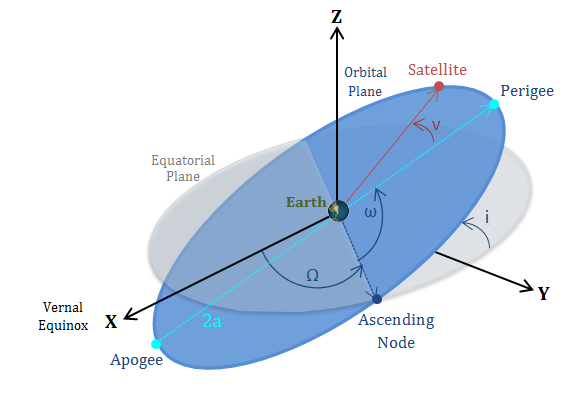
\includegraphics[scale=0.3]{images/COE.png}
}{
  \caption{Classical Orbital Elements} \label{COE}
}
\ffigbox{%
  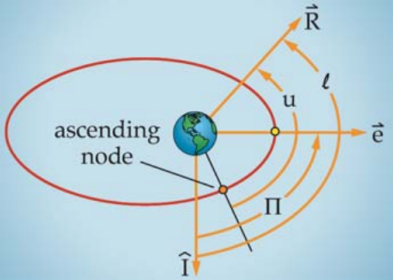
\includegraphics[scale=0.5]{images/AOE.png}
}{
  \caption{Alternate Orbital Elements} \label{AOE}
}
\end{floatrow}
\end{figure}

\large \hspace{-3em}\textbf{Classical Orbital Elements}
\normalsize
\begin{enumerate}
\item \textbf{Semi-major Axis($a$):} This is a constant that defines the size of the orbit. In Circular it is the radius of the circle. It is the longest diameter of an ellipse.
\begin{align}
a&= \dfrac{r_a+r_p}{2}\\
a&=\dfrac{h^2/\mu}{1-e^2}\\
where,\nonumber \\
&r_a = Radius\;of\;Apogee(F_1B)\nonumber\\
&r_p = Radius\;of\;Perigee(F_1A)\nonumber \\
&\mu = Standard\;Gravitational\;Parameter,\nonumber
\end{align}
\item \textbf{Eccentricity($e$):} This the parameter of the conic section which determines its shape. It is defined as the ratio of distance b/w two foci to the Major-axis.
\begin{align}
e&=\dfrac{c}{a}\\
e&=\frac{1}{\mu}\left[\left(\frac{v^2-\mu}{r}\right)\times \overrightarrow{r}-(\overrightarrow{r}.\overrightarrow{v})\times \overrightarrow{v}\right]\label{codeformecc} \\ 
where, \nonumber\\
r_a\;\&\;r_p &= Radius\;of\;Apogee\;\&\;Perigee\;respectively,\nonumber\\
\mu &= Standard\;Gravitational\;Parameter,\nonumber \\
\overrightarrow{v}\;\&\; v &= Velocity\;vector\;\&\;Magnitude\;of\;Velocity\;Vector\;at\;r,\nonumber \\
\overrightarrow{r}\;\&\;r &= Radius\;Vector\;\&\;Magnitude\;of\;Radius\;Vector.\nonumber 
\end{align}
\item \textbf{Inclination($e$)}: It is the tilt of the orbit w.r.t the equatorial plane, measured at ascending node. It can also be defined as the angle from $\hat{K}$ unit vector to the specific angular momentum vector $\vec{h}$.
\begin{align}
i &= \cos^{-1}\left(\dfrac{\overrightarrow{h}.\overrightarrow{K}}{|h|}\right)\\
where,\nonumber \\
\overrightarrow{h}&=Specific\;Angular\;Momentum, \nonumber \\
\overrightarrow{K}&=Unit\;Vector\;in\;Z\;direction, \nonumber  \\
|h|&=Magnitude\;of\;Specific\;Angular\;Momentum. \nonumber
\end{align}
\item \textbf{Right Ascension of Ascending Node($\Omega$):} RAAN horizontally orients the ascending node of the orbit w.r.t the Equatorial plane’s vernal equinox, measured in an equatorial plane This is not defined when the inclination is 0 or 180 degree. It lies between 0 to 360 degrees.
\begin{align}
\Omega &= \cos^{-1}\left(\dfrac{\overrightarrow{I}.\overrightarrow{n}}{|n|}\right)\\
where, \nonumber \\
\overrightarrow{n}&= Nodal\;vector \nonumber\\
It's\;the\;vector\;that\;&joins\;the\;ascending\;node\;and\;the\;descending\;node. \nonumber
\end{align}
\item \textbf{Argument of Perigee($\omega$):} Argument of Perigee defines the orientation of the ellipse in the orbital plane, as an angle measured from the ascending node to the periapsis measure in the direction of the spacecraft’s motion. This is not defined when inclination is 0 or 180 degree or eccentricity is 0. It lies between 0 to 360 degree.
\begin{align}
\omega &= \cos^{-1}\left(\dfrac{\overrightarrow{n}.\overrightarrow{e}}{|n||e|}\right)\\
where, \nonumber\\
\overrightarrow{e}&=Eccentricity Vector. \nonumber
\end{align}
\item \textbf{True Anomaly($\nu$):} True Anomaly defines the position of the spacecraft w.r.t perigee. It’s the angle between the spacecraft and the perigee of the orbit. It lies between 0 to 360 degree. 
\begin{align}
\nu &= \cos^{-1}\left(\dfrac{\overrightarrow{e}.\overrightarrow{r}}{|e||r|}\right)\\
where,\nonumber\\
\overrightarrow{r}&=Radius Vector\nonumber
\end{align}
\end{enumerate}
\large \textbf{Alternate Orbital Elements}
\normalsize
\begin{enumerate}
\item \textbf{Longitude of Perigee($Pi$)} is the angle from the principle direction to perigee. This is used whenever inclination is either 0$^o$ or 180$^o$ as there is no ascending node. It's lies between $0^0$ to $360^0$. In the figure(\ref{AOE}) Longitude of perigee is represented as \enquote{$\Pi$}.
\begin{align}
\Pi = \cos^{-1}\left(\dfrac{\overrightarrow{I}.\overrightarrow{e}}{|e|}\right)
\end{align}
\item \textbf{True Longitude} is the angle from the principle direction to the spacecraft's position. This is used whenever there is no perigee and the the inclination is either $0^0$ or $180^0$. It's lies between $0^0$ to $360^0$. It lies between 0 to 360 degree. In the figure(\ref{AOE})True Longitude is represented as \enquote{$l$}
In the figure(\ref{AOE})True Longitude is represented as \enquote{$l$}. In the figure(\ref{AOE}) Longitude of perigee is represented as \enquote{$\Pi$}.
\begin{align}
l = \cos^{-1}\left(\dfrac{\overrightarrow{I}.\overrightarrow{r}}{|r|}\right)
\end{align}
\item \textbf{Argument of Latitude($u$)} is the angle from ascending to the spacecraft's position. This is used whenever a perigee is absent(i.e., e=0,Circular Orbit). It's lies between $0^0$ to $360^0$.\\
In the figure(\ref{AOE}) Argument of latitude is represented as \enquote{$u$}.
\begin{align}
u = \cos^{-1}\left(\dfrac{\overrightarrow{n}.\overrightarrow{r}}{|n||r|}\right)
\end{align}
\end{enumerate}
\subsection{2D and 3D Orbits}

Based on the inputs given the application can plot either 2D or 3D or both. If the inputs are just Semi major axis and eccentricity or Radius of perigee and apogee or, $r_1,\;v_1,\;\gamma_1$ then the resultant plot will be in the perifocal frame. If the inputs are state and velocity vector or orbital elements then the resultant will be a 3D orbit. 
\begin{table}[H]
\centering
\begin{tabular}{@{}cl@{}}
\toprule
\multirow{2}{*}{\textbf{Inputs}}                      & For 2D - $a,e/r_a,r_p/ r_1, v_1, \gamma_1$ \\ \cmidrule(l){2-2} 
                                             & For 3D - Orbital Elements, State Vectors   \\ \midrule
\multicolumn{1}{r}{\multirow{2}{*}{\textbf{Outputs}}} & Orbit in the Perifocal Frame               \\ \cmidrule(l){2-2} 
\multicolumn{1}{r}{}                         & Orbit in a virtual 3D Environment          \\ \bottomrule
\end{tabular}
\caption{I/O for 2D and 3D orbits}
\label{o23}
\end{table}
There are two ways to plot a orbit, if the plot is on a 2D plane, i.e., Perifocal Plane, the the trajectory equation can be used to plot it easily.
$$r=\dfrac{h^2/\mu}{1 - e\cos(\theta)}$$
If the plot is 3D then solving for the trajectory analytically can be tricky and expensive computing wise depending on the orbit. But, solving it numerically will yeild the orbit with wide range of accuracy depending on the numerical method. The method has mainly two properties to be considered for at this level, the computing speed and the accuracy. A good compromise between these both is desirable for most of the cases. In this case we need a ODE solver. Here are a few types of numerical methods:
\begin{enumerate}
\item Euler Method
\item Backward Euler Method
\item First-order Exponential integrator Method
\item Generalizations
\item Parallel-in-time Methods
\item Integrals over Infinite intervals
\end{enumerate} 
In a programming language based on these methods ODE solvers are written. The most popular ones are:
\begin{enumerate}
\item \textbf{lsoda} - This automatically selects a solver which is appropriate for the given equation.
\item \textbf{lsode} - Since lsoda turns out to be slow, then the DE might need a stiff solver(i.e., very small time steps), this will choose only the stiff solvers 
\item \textbf{ode23} -  Simultaneously uses fourth and fifth order RK formulas to make error estimates and adjust the
time step accordingly. For nonstiff ODEs
\item \textbf{ode45} - Uses simultaneously second and third order Runge Kutta formulas to make estimates of the
error, and calculate the time step size. Since the second and third order RK require less steps, ode23 is
“less expensive” in terms of computation demands than ode45, but is also lower order. Use for nonstiff
ODEs
\end{enumerate}
For MOPy lsoda is sufficient enough for now. So lsoda is used to solve for the acceleration vector. If the acceleration vector is solved twice then we obtailn the position vectors using which a 3D plot can be plotted. The acceleration vector is: 

$$Enter the acceleration vector$$

\subsection{Euler Angle}

The inputs for this are as in table(\ref{eadcm}). This code can be fed the model in 3D environment and the orientation of the model can be manipulated with this.
\begin{table}[H]
\centering
\begin{tabular}{@{}cl@{}}
\toprule
\multirow{2}{*}{\textbf{Inputs}}                      & Directional Cosine Matrix \\ \cmidrule(l){2-2} 
                                             & Euler Angles              \\ \midrule
\multicolumn{1}{r}{\multirow{2}{*}{\textbf{Outputs}}} & Euler Angles              \\ \cmidrule(l){2-2} 
\multicolumn{1}{r}{}                         & Directional Cosine Matrix \\ \bottomrule
\end{tabular}
\caption{I/O for conversion between Euler angle and DCM}
\label{eadcm}
\end{table}
\subsection{Sphere of Influence}
In this section, the user can either input the values or interact with the model in the 3D environment to see the corresponding output.
\begin{table}[H]
\centering
\begin{tabular}{@{}rl@{}}
\toprule
\multicolumn{1}{c}{\textbf{Inputs}} & Minor Body                     \\ \midrule
\multirow{2}{*}{\textbf{Outputs}}   & Radius of SOI in desired units \\ \cmidrule(l){2-2} 
                           & 3D visualization of sphere of influence in virtual environment                         \\ \bottomrule
\end{tabular}
\caption{I/O for Sphere of Influence}
\label{soi}
\end{table}
The sun is the dominant celestial body in the solar system. It has a mass of over 300,000 earths. The sun’s gravitational pull holds all the planets in its hold according to Newton’s law of gravity. However, near a given planet, the influence of its own gravity exceeds that of the sun. For example, at its surface the earth’s gravitational force is over 1600 times greater than the sun’s. The inversesquare nature of the law of gravity means that the force of gravity $F_g$ drops off rapidly with distance r from the center of attraction. If $F_{g0}$ is the gravitational force at the surface of a planet with radius $r_0$, then Figure 8.5 shows how rapidly the force diminishes with distance. At ten body radii, the force is 1$\%$ of its value at the surface. Eventually, the force of the sun’s gravitational field overwhelms that of the planet.

To estimate the planets Sphere of Influence, the three body problem system comprising of planet p of mass MiB\_ mass, the sun s and its mass MaB\_ mass with the distance between then being R and the equation on hand is:
\begin{align*}
r_{SOI}&=R\left(\dfrac{MiB\_ mass}{MaB\_ mass}\right)^{2/5}
\end{align*}

\subsection{Orbital Transfer}
This feature simulates the orbital transfer using various numerical methods. For now, this can perform Hohmann Transfer. The Inputs and outputs are as in table(\ref{tab:ot})
\begin{table}[H]
\centering
\begin{tabular}{@{}cl@{}}
\toprule
\multicolumn{1}{c}{\textbf{Inputs}} & Minor Body, Major Body, Orbital parameters of both initial and final orbit.                     \\ \midrule
\multirow{2}{*}{\textbf{Outputs}}   & Values such as Radius of apogee, Radius of perigee, DeltaV, Time-period of the orbit etc \\ \cmidrule(l){2-2} 
                           & 3D visualization of desired orbital transfer \\ \bottomrule
\end{tabular}
\caption{I/O for Orbital transfer}
\label{tab:ot}
\end{table}
Transfer Orbit is nothing but the path followed by the satellite to travel from an initial orbit to final 
orbit or one planet to other planet. There are many types of transfer orbits in which most commonly used transfer 
is Hohmann Transfer because of its simplicity and its efficient to transfer.
Transfer orbits are:
\begin{enumerate}
\item \textbf{Hohmann Tranfer Orbit: }A Hohmann Transfer is a two-impulse(delta-v) elliptical transfer between two co-planar circular/elliptical orbits. The transfer orbit's apoapsis lies on the target orbit and the periapsis of transfer orbit lies on the initial orbit.The fundamental assumption behind the Hohmann transfer, is that there is only one major body which exerts a gravitational force on the body of interest, such as a satellite. This is most commonly used transfer method for transferring an earth-based satellite from a low orbit to say a geosynchronous orbit.
\begin{figure}[H]
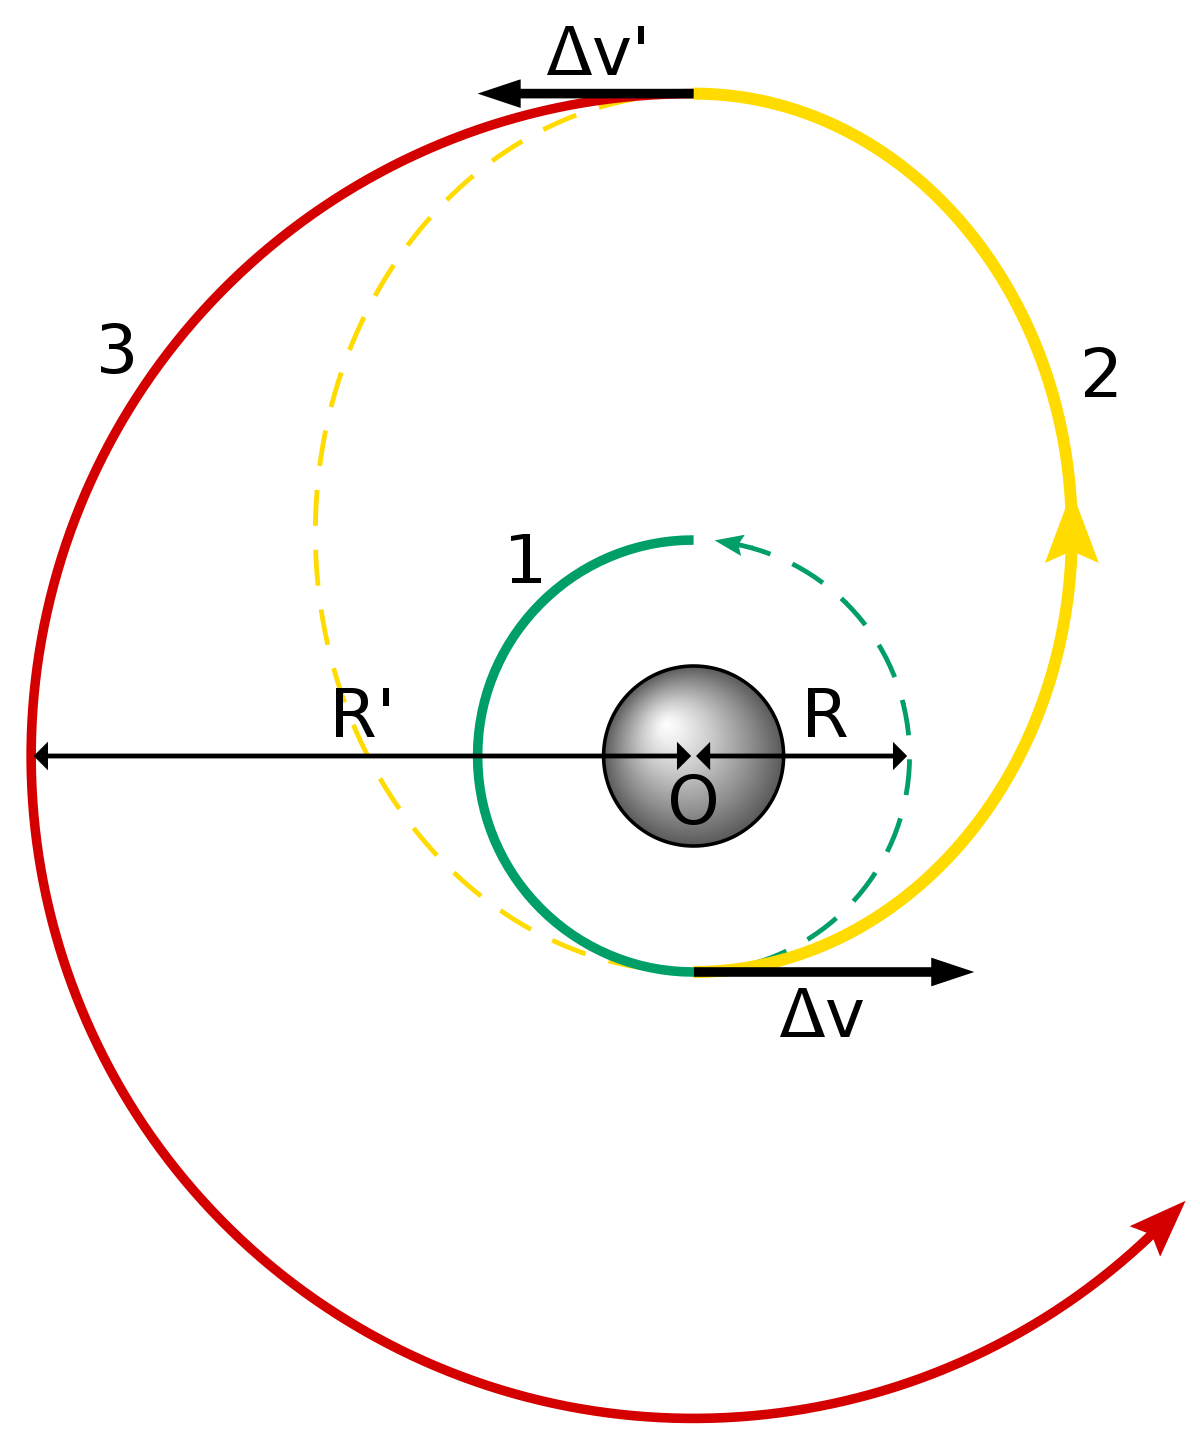
\includegraphics[scale=0.1]{images/ht.png}
\caption{Hohmann Transfer}
\end{figure}
\item \textbf{Bielliptical Transfer Orbit}: In the bi-elliptic transfer, the first transfer is a highly eccentric orbit with an apoapsis higher than the target orbit radius. Once the spacecraft has reached apoapsis, it performs a prograde burn raising its periapsis to the height of its target orbit. Finally, once it reaches periapsis, it performs an orbital insertion burn (Retrograde burn) to put it into a circular orbit. In some cases Bielliptical Transfer is preffered over Hohmann transfer because its
slight fuel efficint transfer.
\begin{figure}[H]
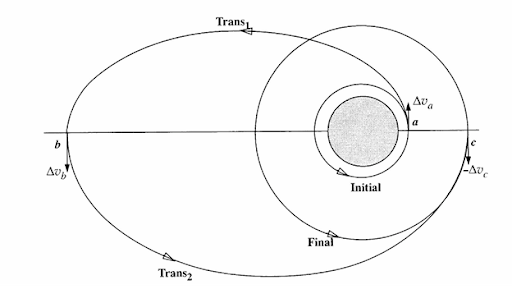
\includegraphics[scale=0.7]{images/bi.png}
\caption{Hohmann Transfer}
\end{figure}
\item \textbf{Low Energy Transfer Orbit:} A low energy transfer is a path in space to reach a target with very little consumption of fuel.
\item \textbf{Constant-Thrust Transfer Orbit:} In this transfer path the spacecraft's engine will be producing constant thrust through out the path. The spacecraft points straight towards the target with constant acceration till it reaches the target. 
\end{enumerate}
\subsection{Calculation of Julian Day}
In this section the user can choose between Gregorian calendar and Julian calendar and with the other inputs they can obtain the Julian day of the corresponding date. 
\begin{table}[H]
\centering
\begin{tabular}{@{}cl@{}}
\toprule
\textbf{Inputs}  & YYYY-MM-DD , hh:mm:ss, Type of calender \\ \midrule
\textbf{Outputs} & Julian-day  \\ \bottomrule                                              
\end{tabular}
\caption{I/O for Julian-day}
\label{tab:jd}
\end{table}
The Julian day is the continuous count of days since the beginning of the Julian period i.e., January 1, 4713 B.C. at 12 Noon, and is used primarily by astronomers for easily calculating elapsed days between two events.
To calculate a Julian Day there are many formulae, but the generalised formula is:\\
To convert from Gregorian calendar:
\begin{multline*}
JDN = \dfrac{1461\left(Y+4800+\dfrac{M-14}{12}\right)}{4}+\dfrac{367\left(M-2-12\dfrac{M-14}{12}\right)}{12} - \\
\dfrac{3\left( \dfrac{Y+4900+\dfrac{M-14}{12}}{100}\right))}{4}+D-32075
\end{multline*}
To convert from Julian Calendar:
$$JDN = 367 \times Y - \dfrac{7 \left( Y+5001+\dfrac{M-9}{7}\right)}{4}+\dfrac{275M}{9}+D+1729777$$
Once the Julian Day Number is obtained the time is taken into account. So, The Julian day becomes:
$$JD = JDN+\dfrac{HH-12}{24}+\dfrac{MM}{1440}+\dfrac{SS}{86400}$$
\subsection{Calculation of Parameters of the Orbit}
The user can obtain various parameters by giving the details that they know of. If necessary they can plot the orbit too.
\begin{table}[H]
\centering
\begin{tabular}{@{}rl@{}}
\toprule
\multicolumn{1}{c}{\textbf{Inputs}} & $a,e/r_a, r_p/r_1,\;v_1,\;\gamma_1$/ Orbital Elements/State and velocity vectors \\ \midrule
\multirow{2}{*}{\textbf{Outputs}}   & $\mu,\;,h\;,\epsilon$, Forces and Velocity at significant position               \\ \cmidrule(l){2-2} 
                           & Mean Motion, Time Period                                                         \\ \bottomrule
\end{tabular}
\caption{I/O for Various Parameters of the Orbit}
\label{vpco}
\end{table}
The Semi major axis ,Eccentricity, Radius of perigee, Radius of apogee, Specific mechanical energy, Specific angular momentum, Time period , Mean motion, Velocity at perigee, Velocity at apogee, Gravitational force at perigee, Gravitational force at apogee, Semi-latus rectum, Velocity at semi-latus rectum, Escape velocity at perigee and Escape velocity at apogee all these parameters can be calculated. These parameters can be calculated at any given point of time in the ongoing mission.
The major formula used in it are:\\

% Please add the following required packages to your document preamble:
% \usepackage{multirow}
\begin{table}[H]
\centering
\begin{tabular}{ccc}
\
\textbf{Circular and Elliptical}           & \textbf{Parabolic}               & \textbf{Hyperbolic}                             \\ \hline
\multicolumn{3}{c}{$\mu=G\times M_{Major}$}                                                                                                                               \\ 
\multicolumn{1}{c|}{$r_p=a\times (1-e)$}                        & \multicolumn{1}{c|}{\multirow{2}{*}{$l=2\times r_p$}} & $\theta_\infty = \cos^{-1}(\dfrac{1}{e})=\beta$ \\
\multicolumn{1}{c|}{$r_a=a\times (1+e)$}                        & \multicolumn{1}{c|}{}                                 & $\delta = 2\sin(\dfrac{1}{e})$                  \\
\multicolumn{1}{c|}{$\epsilon = \dfrac{-\mu}{2a}$}              & \multicolumn{1}{c|}{$0$}                              & $h=\sqrt{\mu a(e^2-1)}$                         \\
\multicolumn{1}{l|}{}                                           & \multicolumn{1}{l|}{}                                 & \multicolumn{1}{l}{}                            \\
\multicolumn{1}{c|}{$h=\sqrt{r_p\times(1+e)\mu}$}               & \multicolumn{1}{c|}{$h=\sqrt{2\mu r_p}$}              & $b=ae\sin(\theta_\infty)=\Delta$                \\
\multicolumn{1}{l}{}                                            & \multirow{2}{*}{$F_g=\dfrac{GMm}{r^2}$}               & \multicolumn{1}{l}{}                            \\
                                                                &                                                       &                                                 \\
\multicolumn{1}{c|}{$V= \sqrt{\dfrac{2\mu}{r}-\dfrac{\mu}{a}}$} & \multicolumn{1}{c|}{$V_r=\sqrt{\dfrac{2\mu}{r}}$}     & $V_\infty=e\mu\sin(\theta_\infty)/h$            \\
\multicolumn{1}{c|}{$T = \sqrt{\dfrac{4\pi^2}{\mu}\times a^3}$} & \multicolumn{1}{c|}{}                                 & $\epsilon=\dfrac{\mu}{2a}$                      \\
\multicolumn{1}{c|}{$n = \dfrac{2 \pi}{T}$}                     & \multicolumn{1}{c|}{}                                 & $l=\dfrac{-b^2}{a}$                             \\
\multicolumn{1}{c|}{$l=a\times(1-e^2)$}                         & \multicolumn{1}{c|}{}                                 & $r_p,r_a = \dfrac{h^2/\mu}{1 \pm e}$           
\end{tabular}
\caption{Formulae for Various parameters}
\label{tab:vpco}
\end{table}
\subsection{Sensitivity Analysis}
User has to select the type of calendar and the in the input section they have to select date and time and accuracy of digits and then by clicking on calculate button we will get Julian days in the output section. This takes in the required values an outputs how much of an error will that small change in the velocity or radius in the 3D environment.

\begin{table}[H]
\begin{tabular}{@{}cl@{}}
\toprule
\textbf{Input}  & State Vector, Velocity Vector and two delta-v with slight difference                                                                      \\ \midrule
\textbf{Output} & \begin{tabular}[c]{@{}l@{}}Percentage difference caused to the final orbit parameters due to slight \\ difference in delta-v\end{tabular} \\ \bottomrule
\end{tabular}\caption{I/O for Sensitivity Analysis}
\end{table}
The analysis is done to know what is the effect, if small error occurs in position and velocity at the maneuver point while the space mission is on the trajectory. There is a derived formula to calculate the sensitivity analysis from which change in position and velocity can be obtained in terms of percentage . This helps in analysing the position and velocity tolerance of any particular mission and design accordingly.
\subsection{Position of One Spacecraft Relative To Another}
Based on the inputs of the user the relative velocity and orbit can be visualized in this section.
\begin{table}[H]
\begin{tabular}{@{}cl@{}}
\toprule
\textbf{Input}  & Major Body, State Vector and Velocity Vector of Minor Body    \\ \midrule
\textbf{Output} & Graph Showing the Minor bodies in the orbit around Major Body \\ \bottomrule
\end{tabular}\caption{I/O for Position of One Spacecraft Relative To Another}
\end{table}

In situations like a rendezvous maneuver the relative motion between the space vehicles is utilised. This can be done in two different ways, utilising the algorithm to calculate the relative orbit or utilise the camera viewpoint and plotting as the orbit propagates with the camera fixed on one of the spacecraft.
\subsection{Lagrangian Points}
The Lagrangian points are points near two large orbiting bodies, the two objects exert an unbalanced gravitational force at a point, altering the orbit of whatever is at that point. At the Lagrange points, the gravitational forces of the two large bodies and the centrifugal force balance each other, The inputs and outputs are as follows.
\begin{table}[H]
\begin{tabular}{@{}cc@{}}
\toprule
\textbf{Input}  & Major Body, Minor Body and Distance Between them           \\ \midrule
\textbf{Output} & Lagrangian points polar coordinates and Graph showing them \\ \bottomrule
\end{tabular}\caption{I/O for Lagrangian Points}
\end{table}
    Lagrange Points are positions in space around the planet/star, where the gravitational forces of two body like 
the Sun and the Earth produce enhanced regions of attraction and repulsion. These can be used by spacecraft to reduce fuel 
consumption required to remain in position. At these points gravitational pull of two large masses precisely equals the centripetal 
force required for a small object to move with them.
    These points are named in honor of Italian-French mathematician Josephy-Louis Lagrange. There are five Langrengian 
points around the planet/satr, where a small mass can orbit in a constant pattern with two larger masses.  This mathematical 
problem, known as the "General Three-Body Problem" was considered by Lagrange in his prize winning paper (Essai sur le Problème des 
Trois Corps, 1772).
    Of the five Lagrange points, three are unstable and two are stable. The unstable Lagrange points - labeled L1, L2 and L3 - lie along 
the line connecting the two large masses.The three of them lie along the line connecting the two large bodies.
The stable Lagrange points - labeled L4 and L5 - form the apex of two equilateral triangles 
that have the large masses at their vertices. L4 leads the orbit of earth and L5 follows.